\chapter{绪论}

\section{研究背景与意义}

在全球战略格局深刻调整与新一轮科技革命加速演进的背景下,空天领域已成为衡量国家综合实力和维护国家安全的核心战略疆域~\cite{X}。确保我国在空天领域的安全、自主与战略主动,对于实现国家现代化发展目标具有不可替代的基础性作用。空天技术的飞速发展催生了数量庞大、性能先进、行为模式多样的新型空天目标,如高超声速飞行器~\cite{X}、大规模低轨卫星星座~\cite{X}、隐身作战平台及无人机集群~\cite{X}等。这些目标普遍具有的高动态、低可探测、智能化和网络化特征,对现有国家防空预警、空间态势感知乃至整体空天防御体系的有效性构成了前所未有的挑战,显著增加了对其进行可靠探测、跟踪、识别与处置的复杂性和难度~\cite{X}。

面对此严峻态势,发展先进的空天目标识别能力,实现对各类目标的及时发现、稳定跟踪、精确分类与可靠评估,已成为构筑坚实国家空天安全屏障、支撑高效军事行动与明智战略决策的核心要素~\cite{X}。精确的目标识别是有效拦截、精确打击、威胁评估、意图判断等一系列后续行动的基础。缺乏准确的目标属性信息,将导致空天态势认知模糊,指挥控制效能下降,信息优势难以确立。尤其是在现代战争所特有的复杂电磁环境和高强度对抗条件下,能否快速、准确地判明目标的具体类型、型号乃至身份,直接关系到作战资源的优化配置、战场迷雾的有效驱散以及战略误判风险的管控~\cite{X}。近期如俄乌冲突与巴以冲突等局部战争的实践,更是直观地展示了在无人平台、精确制导弹药和先进传感器广泛应用的现代战场上,空天目标精确识别能力对于实时战场态势生成、作战效果评估乃至冲突走向的关键性影响。准确识别敌方高价值节点(如指挥控制中心、关键传感器)和主要威胁(如来袭导弹、攻击无人机),已成为夺取战场主动权、提升作战效能的核心环节。因此,先进的目标识别技术已成为现代军事体系不可或缺的关键技术支撑。

鉴于空天目标识别的极端重要性,世界主要国家均将其置于国防科技发展的优先地位~\cite{X}。美国凭借其强大的研发体系,持续投入于先进传感器、智能信息处理及网络化监视系统的建设,特别是在人工智能(尤其是深度学习)应用于目标识别领域保持领先~\cite{X}。欧洲国家通过多边合作,在高性能雷达、卫星侦察和多源融合技术方面不断取得进展~\cite{X}。俄罗斯等国则在应对特定威胁(如高超声速目标)和复杂对抗环境下的识别技术上展现其特色。各国研究的共同焦点在于如何克服目标信号微弱、动态性强、背景扰动复杂、目标类型多样及智能化对抗等技术难题,并积极利用人工智能、大数据、多传感器协同等新兴技术,实现对空天目标的{全域、全时、全谱}精确感知与深度认知~\cite{X}。

对于我国而言,维护国家统一、保障领土完整、拓展海外利益以及推进海洋强国、航天强国等战略目标的实现,均对空天态势感知与目标识别能力提出了极高要求~\cite{X}。我国面临的空天安全环境复杂,潜在威胁来源多样,涵盖从高性能隐身平台、战略武器,到临近空间与轨道空间的新型飞行器、各类卫星,再到低小慢无人机等不同维度~\cite{X}。若无法对这些潜在威胁进行有效识别,国家空天预警防御体系将存在关键短板,直接威胁国家安全。同时,随着国家利益的全球化和自身空天活动的日益频繁(如空间站运营、北斗全球服务、密集卫星部署、繁忙民航交通等),保障海外利益和自身空天资产安全的需求也日益凸显。准确识别空间碎片、非合作接近目标或攻击威胁,是维护我国空天基础设施稳定运行、支撑经济社会发展的重要保障~\cite{X}。因此,发展自主可控、国际先进的空天目标自动识别技术体系,全面提升精确识别与深度理解能力,不仅是应对现实安全挑战的迫切需要,更是支撑国家重大战略、提升综合国力的基础工程。攻克非合作目标精确识别等技术难题,是我国国防科技领域必须抢占的战略制高点。本研究正是立足于此重大战略需求,聚焦于空天目标识别技术链中的核心挑战,旨在通过深入研究为提升我国在该领域的自主创新能力提供理论与技术支撑。

在空天目标探测识别的多种技术手段中,雷达系统凭借其独特的物理原理和工程优势,长期以来在空天感知体系中扮演着核心角色,并预计在未来仍将保持其骨干地位~\cite{X}。作为主动探测设备,雷达的核心优势首先体现在其{全天候、全天时}的工作能力,电磁波传播基本不受光照、云、雾、雨、雪等气象条件限制,确保了探测系统的连续性和可靠性,这与依赖环境条件的光学、红外等被动手段形成鲜明对比~\cite{X}。其次,雷达通常具备{作用距离远、覆盖范围广}的特点,能够对广阔空域或空间进行有效搜索与监视,为后续处理提供必要的预警时间~\cite{X}。更为关键的是,雷达不仅能精确测量目标的距离、方位、速度等运动学参数,还能通过精细分析回波信号的{幅度、相位、频率、极化}等特征,反演目标的{物理属性}(如尺寸、形状、结构、材质)和{精细运动状态}(如姿态、微动),为非合作目标的精确识别提供了不可或缺的信息来源~\cite{X}。

现代雷达技术的进步,特别是宽带信号处理和高分辨率成像技术的发展,极大地提升了雷达获取目标细节信息的能力~\cite{X}。宽带信号的应用提高了距离分辨率,能够分辨目标沿雷达视线(Line of Sight,LOS)的散射中心分布,形成{高分辨率距离像(High Resolution Range Profile,HRRP)}~\cite{X}。HRRP蕴含了目标一维结构信息,是雷达自动目标识别(Radar Automatic Target Recognition,RATR)研究中最常用的一类特征~\cite{X}。同时,{合成孔径雷达(Synthetic Aperture Radar,SAR)}~\cite{X}与{逆合成孔径雷达(Inverse-SAR,ISAR)}~\cite{X}等成像技术能够生成目标的二维甚至三维高分辨率图像,直观展示其几何形态和散射点布局,为识别提供了更丰富的信息。这些高分辨率技术的发展,为RATR技术奠定了基础,使其成为提升空天态势感知智能化水平的关键途径~\cite{X}。回顾其发展历程,RATR技术大致经历了从早期的{模板匹配}~\cite{X},到中期的{特征工程与浅层分类器}~\cite{X},再到近十余年来由{深度学习}驱动的新阶段~\cite{X}。深度神经网络凭借其强大的{自动特征学习}和{非线性建模}能力,实现了“端到端”的识别,在数据充足时显著超越了传统方法,成为当前研究的主流范式。国际主要研究机构均在积极探索深度学习在RATR各方向(如SAR及ISAR图像分类、HRRP序列识别、微多普勒分析)的应用~\cite{X}。

然而,尽管深度学习带来了巨大进步,但将其成功应用于实际复杂环境的RATR仍面临源于物理限制和应用场景复杂性的严峻挑战~\cite{X}。{一方面,雷达目标特征的内在复杂性与对观测条件的极端敏感性依然是核心难题~\cite{X}。} 电磁散射过程受多重因素耦合影响,导致雷达特征(特别是HRRP)对目标姿态角变化极为敏感(即{“姿态敏感性”}),微小变动即可引起特征剧烈畸变,严重影响识别稳定性~\cite{X}。SAR等二维像同样存在角度依赖性,且成像质量受运动状态影响~\cite{X}。目标微动引入的微多普勒效应进一步增加了信号的复杂度。因此,从复杂、时变、敏感的雷达信号中提取稳定且具判别力的特征表示,始终是RATR领域的核心科学问题。{另一方面,真实电磁环境中的噪声、杂波是制约RATR实际性能的关键障碍~\cite{X}。} 雷达信号不可避免地混杂背景杂波(地杂波、海杂波、气象杂波),这些{噪声和杂波}严重降低了信号质量,污染甚至淹没目标特征,对后续处理造成极大困难。如何在低信噪比条件下实现{稳健识别},是衡量RATR系统实用价值的关键指标。

{此外,当前最为突出的瓶颈是高质量、大规模、标注完备的训练数据普遍严重匮乏,即“小样本问题”~\cite{X}。} 深度学习的性能高度依赖大数据训练,但在RATR领域,获取此类数据的成本高昂、限制众多(实测获取难)、目标类型动态变化(数据库难完备)、状态多样性导致样本需求巨大、数据标注困难且昂贵、仿真数据与实测数据间存在显著“域差异”(Domain Gap)等因素共同导致了训练样本的稀缺~\cite{X}。这种数据稀缺性与深度模型的数据需求之间的矛盾,构成了当前RATR发展的核心困境。在小样本条件下,深度模型极易{过拟合},导致{泛化能力}严重不足。因此,研究如何在有限标注样本下实现高效、可靠的识别,提升模型的泛化性和对新目标的快速适应能力,已成为推动RATR技术走向实用化的关键突破口。

{最后,现有方法在利用目标语义信息方面尚显不足。} 多数方法依赖底层物理特征,而目标本身蕴含的{语义信息}(如类别、功能、型号、威胁等级等)对于区分相似目标、理解意图、辅助决策具有重要价值~\cite{X}。在小样本或低分辨条件下,对于物理特征目标区分度不足的情况,融合语义信息有望提升识别精度和可靠性。然而,如何有效表示、融合跨模态的物理特征与语义信息,并将其整合到学习与推理过程中,仍是待深入探索的研究方向。

面对上述局限与挑战,RATR技术呈现出以下主要发展趋势:一是持续追求更高质量的特征信息获取(更高分辨率~\cite{X}、更精细特征~\cite{X});二是发展更智能、适应性更强的识别模型(深度学习与雷达特性深度融合,如时空建模~\cite{X}、自监督~\cite{X}、持续学习~\cite{X});三是显著提升模型在复杂环境下的鲁棒性(抗噪抗扰设计~\cite{X},物理知识引导的机器学习~\cite{X});四是{集中力量攻克小样本学习难题},其中,以{元学习(Meta-Learning)}为代表的“学会学习”范式,因其在快速适应新任务、提高样本效率方面的潜力而备受关注~\cite{X},是本论文的核心研究方法;五是积极探索多源信息融合与协同识别~\cite{X};六是日益关注模型的可解释性、可信赖性与安全性~\cite{X}。

综上所述,RATR技术的发展机遇与挑战并存。以深度学习为代表的AI技术注入了新活力,但也使其在数据依赖(特别是小样本困境)、环境适应性、特征复杂性等方面面临严峻制约。有效解决小样本学习问题,提升模型在真实复杂环境下的鲁棒性、泛化能力和快速适应能力,是当前RATR领域亟待突破的核心技术瓶颈。本研究正是围绕此瓶颈,以元学习为主要理论框架,深入研究其在解决小样本雷达HRRP目标识别问题中的应用潜力,特别是在应对噪声扰动、角度敏感性和语义信息利用等具体技术难点方面,提出针对性的创新方法,旨在为提升我国空天目标精确识别技术水平提供理论与技术储备。

\section{空天目标RATR技术研究现状}
前文深入探讨了空天目标精确识别的战略紧迫性,并分析了雷达作为核心传感手段的优势、局限及发展趋势,特别指出了“小样本问题”是制约当前先进识别算法性能的关键瓶颈。在此基础上,本节将进一步聚焦于RATR领域如何应对数据稀缺性的挑战。我们将首先回顾传统RATR方法为何在处理复杂性和小样本问题上存在固有的局限性;接着,阐述深度学习方法如何作为一种更强大的范式被引入RATR领域,并分析其在带来性能提升的同时,如何使得小样本问题变得更为突出和关键;最后,在此背景下,系统梳理当前专门针对小样本RATR的研究现状、主要技术途径及其面临的持续挑战。

在深度学习技术广泛应用之前,RATR的研究主要沿着两条技术路径发展:基于模板匹配~\cite{X}和基于特征工程与浅层分类器~\cite{X}。模板匹配方法通过将待测目标特征与预建模板库进行比对来识别,原理直观,但在面对目标多样性、姿态剧变以及模板库难以完备的现实时,尤其是在可用样本稀少、无法构建代表性模板库的小样本条件下,其性能和鲁棒性显著不足~\cite{X}。为了克服这些限制,研究转向了特征工程路线,即人工设计对特定变化(如姿态、噪声)相对不敏感的稳健特征,再结合SVM、KNN等浅层分类器进行判决~\cite{X}。这种方法通过特征提取实现了信息抽象,提升了一定的灵活性和鲁棒性。然而,其成功严重依赖于特征设计的质量,并且需要深厚领域知识、耗时费力且泛化能力有限。特别是在小样本条件下,缺乏足够数据指导特征设计与验证,难以获得真正具有普适判别力的特征~\cite{X}。同时,浅层分类器有限的模型容量也难以充分捕捉雷达数据内在的高度非线性复杂关系,限制了识别性能的上限~\cite{X}。因此,尽管传统方法为RATR奠定了基础,但它们在特征表示能力、模型泛化性、自动化程度以及应对小样本挑战的能力上均存在明显瓶颈,难以满足现代空天目标识别任务对高精度、高鲁棒性、高适应性的需求~\cite{X}。

{传统方法的上述局限性,特别是其在特征表示学习上的不足和对人工经验的过度依赖,自然而然地推动了研究界寻求更强大的数据驱动模型~\cite{X}。深度学习凭借其从大规模数据中自动学习层次化特征表示的卓越能力,在计算机视觉等领域取得革命性成功后,也被迅速引入RATR领域~\cite{X}。以卷积神经网络(Convolutional Neural Network,CNN)~\cite{X}、循环神经网络(Recurrent Neural Network,RNN)~\cite{X}及其变种~\cite{X}、长短时记忆网络(Long-Short Term Memory,LSTM)~\cite{X}、图神经网络(Graph Neural Network, GNN)~\cite{X}以及近年备受关注的Transformer架构~\cite{X}为代表的深度模型,能够直接处理雷达二维像(SAR或ISAR)或序列数据(HRRP),实现了“端到端”的识别流程,在数据相对充分的条件下,展现出超越传统方法的性能潜力~\cite{X},标志着RATR技术进入了一个新的发展阶段。

然而,深度学习的强大性能与其大规模标注数据驱动的特性是一体两面~\cite{X}。虽然RATR领域的数据稀缺问题由来已久,但在深度学习范式下,这个问题变得尤为尖锐和关键。深度模型通常包含数百万甚至更多的参数,需要海量的、多样性的标注样本进行有效训练才能避免过拟合,学习到具有良好泛化能力的特征表示~\cite{X}。但在RATR领域,如前文(1.1.2节)所述,获取大规模、高质量、标注完备的实测数据面临着成本、限制、目标多样性、状态多变性、标注难度以及仿真数据域差异等多重现实障碍。这种深度模型对数据的强依赖性与雷达数据获取的固有困难之间的矛盾,使得{小样本问题从一个普遍存在的挑战,升级为制约深度学习RATR技术实用化、发挥其全部潜力的核心瓶颈}。直接将标准深度学习模型应用于典型的雷达小样本场景,往往导致模型训练不足、过拟合严重,识别性能远达不到预期。因此,如何在深度学习框架下有效应对数据稀缺性,成为RATR领域亟待解决的关键科学问题,直接催生了针对性的{小样本学习(Few-Shot Learning, FSL)}研究方向~\cite{X}。

% ... (保持 1.1 节和 1.2.1 节内容不变) ...

\section{小样本RATR技术面临的挑战}
% 调整本小节开头,明确先总后分
面对传统方法的局限以及深度学习范式下凸显的小样本瓶颈,FSL已成为推动RATR技术发展的关键研究方向~\cite{X}。FSL旨在使模型具备从极少量标注样本中学习并泛化到新类别或新任务的能力~\cite{X}。近年来,研究者们已将多种源于通用机器学习领域的FSL策略引入小样本RATR研究,并针对雷达数据的特性进行了初步的适应与发展。本小节将首先概述这些主流技术途径在RATR领域的应用现状,然后重点剖析本研究所关注的三个核心挑战及其现有研究的不足之处。

% 概述主流FSL方法在RATR中的应用现状
当前应用于小样本RATR的主流FSL技术途径大致可分为以下几类:

{一是基于数据增广(Data Augmentation)的策略~\cite{X}。} {作为缓解数据不足最直接的手段,数据增广通过变换现有样本或生成新样本来扩充训练集。在RATR领域,除了应用旋转、平移等几何变换(需注意保持物理意义,尤其对HRRP等非图像数据)和添加模拟噪声外,基于深度生成模型(如生成对抗网络GANs、变分自编码器VAEs)的样本合成受到了广泛关注。例如,已有研究利用GANs生成逼真的SAR图像~\cite{X}或HRRP样本~\cite{X},以扩充小样本训练集。西安电子科技大学的研究学者在利用GAN进行雷达数据增广方面进行了深入探索~\cite{X}。然而,数据增广的局限性在于:简单变换难以模拟雷达数据(尤其是HRRP)对姿态等因素的复杂、非线性变化;生成模型的训练本身也需要一定数据基础,且生成样本的质量(逼真度、多样性)和与真实数据分布的一致性难以完全保证,尤其对于结构复杂、细节丰富的雷达特征,GANs可能面临模式坍塌等问题~\cite{X};更重要的是,增广数据并未带来关于新类别目标的本质信息,对于提升模型对全新类别的泛化能力帮助有限,其主要作用在于提升模型在已有类别上的鲁棒性和减少过拟合~\cite{X}。}

{二是基于迁移学习(Transfer Learning)与领域自适应(Domain Adaptation)的策略~\cite{X}。} {迁移学习试图将在数据丰富的源域(如大规模仿真数据集、相关实测数据集)上学到的知识(如预训练模型参数)迁移至数据稀缺的目标域。常见的做法是在源域预训练深度模型,然后在目标小样本数据集上进行微调(Fine-tuning)。这种方法能够利用源域的通用特征表示,加速学习并可能提升小样本性能。例如,研究人员尝试利用仿真数据预训练的模型迁移到实测数据识别任务中~\cite{X}。然而,其有效性高度依赖于源域与目标域的相关性。雷达应用中常见的显著“域偏移”(Domain Shift),如仿真与实测之间、不同雷达参数或环境条件之间,会严重限制迁移效果,甚至导致负迁移~\cite{X}。领域自适应技术致力于显式地减小域间分布差异,例如通过对齐特征分布~\cite{X}或利用对抗学习进行域混淆~\cite{X},以提升模型跨域泛化能力。国防科技大学、电子科技大学等单位在雷达信号处理的迁移学习和领域自适应方面均有深入的研究积累~\cite{X}。尽管这些方法在一定程度上缓解了小样本问题,但它们通常假设目标域仍有一定量(可能未标注)的数据可供适应,对于仅有极少量标注样本(如one-shot)的极端小样本场景或需要快速识别在源域中完全未出现过的新类别的情况,其能力仍然受限~\cite{X}。}

{三是基于元学习(Meta-Learning)的策略,其中亦包含度量学习的思想~\cite{X,X}。} {元学习,或称“学会学习”,被认为是解决小样本问题的更根本性范式。它旨在让模型掌握一种通用的学习策略或获得一个良好的初始状态(元知识),使其能在仅有少量标注样本的新任务上快速适应并有效泛化~\cite{X}。元学习通常采用“任务式”训练框架(元训练),通过优化模型在大量模拟小样本任务上的性能来学习元知识。根据学习元知识的方式,主要可分为:
(1) \emph{基于优化的元学习}:如模型无关元学习(Model-Agnostic Meta-Learning,MAML)~\cite{X}及其变种,目标是学习一个对新任务数据极其敏感、只需少量梯度更新即可快速适应的模型初始化参数。已有研究初步将MAML应用于小样本SAR图像分类~\cite{X}。
(2) \emph{基于度量的元学习}:这类方法的核心思想是学习一个通用的嵌入空间或相似度度量函数,使得在该空间中,同类样本紧密聚集,异类样本相互分离。这使得模型能够基于与少量支持集样本的距离或关系来进行预测。原型网络(Prototypical Networks,ProtoNet)~\cite{X}、匹配网络(Matching Networks,MN)~\cite{X}、关系网络(Relation Networks,RelationNet)~\cite{X}等是其中的代表。这些方法因其简洁有效和天然的小样本适应性而备受关注。例如,原型网络通过计算支持集样本在嵌入空间中的类别原型(均值),然后将查询样本归类到最近的原型,已被尝试应用于小样本HRRP识别~\cite{X}和SAR图像识别~\cite{X}。复旦大学等高校在度量学习理论与应用方面有较多研究~\cite{X}。将度量学习视为元学习的一种重要实现途径(学习通用的度量函数作为元知识)是当前的一个普遍观点。
元学习提供了一个系统性的解决小样本问题的框架,其“学会学习”的思想与RATR需要快速适应新目标、新环境的需求高度契合,展现出巨大的应用潜力。}

{挑战一:低信噪比与复杂噪声扰动下的鲁棒识别。}
雷达信号在传播和接收过程中极易受到各种噪声(热噪声、散粒噪声等)、杂波(地、海、气象杂波)的影响,导致目标信号信噪比(SNR)或信杂比(SCR)显著降低~\cite{X}。在小样本条件下,模型本就难以从有限数据中学习到目标的本质特征,噪声的存在进一步模糊了目标信息,引入了虚假特征,显著加剧了特征提取的困难和模型过拟合的风险,导致识别性能急剧恶化。虽然传统方法中有基于统计特性或信号子空间的抗噪声特征设计~\cite{X},深度学习中也有一些研究关注于设计鲁棒网络结构(如引入残差连接~\cite{X}、注意力机制~\cite{X})或采用去噪自编码器等进行预处理~\cite{X},但这些方法往往存在局限:它们通常假设噪声模型已知或相对简单(如高斯白噪声),或者需要足够的数据来学习噪声的统计特性或训练去噪模型。然而,雷达面临的真实噪声往往是复杂、非平稳、甚至未知的,其强度和类型可能随时间、空间动态变化。
现有的通用FSL方法,包括数据增广(简单添加噪声难以模拟真实复杂噪声)、迁移学习(源域可能无噪声或噪声类型不同)、以及元学习及度量学习,大多在相对干净的数据集上进行验证,普遍缺乏针对雷达领域常见的、强度未知或变化、类型复杂的噪声扰动环境进行鲁棒性设计的内禀考量~\cite{X}。例如,标准的元学习任务构建通常不显式模拟噪声水平的变化,学习到的快速适应能力可能对噪声变化不鲁棒;度量学习所学习的嵌入空间可能对噪声扰动非常敏感,导致同类样本在噪声下距离变大,异类样本距离变小。因此,如何在{样本极其有限}的情况下,使模型具备对{未知或变化的噪声}的自适应鲁棒识别能力,是一个亟待解决的关键难题。目前,专门针对{小样本RATR的噪声鲁棒性}研究相对不足,缺乏能够有效应对未知复杂噪声环境的系统性解决方案~\cite{X}。北京理工大学在复杂电磁环境下雷达信号处理方面有较多积累~\cite{X},但将其与小样本学习特别是元学习深度结合的研究尚待深入。

{挑战二:雷达特征(尤其是 HRRP)的角度敏感性。}
雷达回波特性,特别是HRRP,对目标的观测姿态角(方位角、俯仰角)表现出极端敏感性~\cite{X}。这是由雷达散射的物理机制决定的:HRRP是目标散射中心沿雷达视线的一维投影,姿态角的微小变化会导致视线方向的改变,从而引起散射中心投影位置、遮挡关系以及相对强度的剧烈、非线性变化。这种现象使得同一目标在不同角度下的HRRP样本形态可能差异巨大,甚至超过不同目标之间的差异,严重违反了许多机器学习算法(包括FSL)关于“类内紧凑、类间分离”的基本假设~\cite{X}。这一物理瓶颈是RATR,尤其是基于HRRP识别的固有核心挑战。传统方法尝试通过设计角度不敏感特征(如基于旋转不变量的特征)~\cite{X}或建立覆盖宽角度范围的多姿态模板库~\cite{X}来应对,但前者往往以牺牲大量判别信息为代价,导致识别性能下降;后者则面临模板库构建成本高昂、存储量巨大、匹配效率低以及对未覆盖角度泛化能力差等问题。
深度学习方法,例如使用RNN~\cite{X}或LSTM~\cite{X}处理HRRP序列以捕捉角度变化的时序依赖性,或者设计特定的CNN结构(如角度分离网络)~\cite{X},试图学习角度不变表示或显式建模角度变化规律。然而,在小样本条件下,模型难以从有限的、可能角度覆盖不连续的样本中充分学习到这种复杂的、高度非线性的角度依赖关系,导致跨角度泛化能力差,即在训练时未见过或样本稀少的角度范围上识别性能急剧下降~\cite{X}。现有的通用FSL方法,无论是基于优化还是基于度量,通常假设任务内或类别内的样本具有一定的内在相似性。雷达目标的强角度敏感性恰恰打破了这一假设,使得直接应用这些方法效果受限。虽然已有少量工作尝试将FSL应用于跨角度雷达目标识别~\cite{X},例如南京航空航天大学的研究人员可能探索过相关问题~\cite{X},但这些研究可能未能充分挖掘和利用样本间的角度关联信息(如角度连续性、对称性等物理先验),或者在角度跨度较大、样本极其稀疏的极端小样本场景下性能下降仍然显著。因此,如何在{小样本约束}下,有效克服HRRP等雷达特征的{强角度敏感性},实现对{宽角度范围或未知角度}目标的可靠识别,是小样本RATR领域亟待攻克的另一个核心技术挑战。

{挑战三:小样本下特征判别性不足与语义信息利用匮乏。}
当每类目标的训练样本极少时(例如one-shot或few-shot),模型仅能接触到目标极其有限的观测实例。此时,单纯依赖从雷达物理信号(如HRRP的幅度、相位,SAR或ISAR图像的像素强度)中通过深度网络学习到的底层特征表示,可能不足以有效地区分那些结构相似、雷达散射特性接近的不同目标类别~\cite{X}。这种由于样本稀疏导致的{特征判别性不足}问题,在高相似度目标混杂的识别场景中尤为突出。在这种情况下,目标的{语义信息},即关于目标的高层抽象知识,如其所属的功能类别(例如,战斗机、轰炸机、预警机、运输机)、具体型号家族、甚至依据先验情报判断的威胁等级等,能够提供独立于物理特征的重要补充判别线索。例如,两款在HRRP或SAR图像上看起来相似的飞机,可能分属不同的功能类别,具有迥异的作战用途和威胁程度。如果能在识别决策中有效融入这些语义信息,即使物理特征区分度不高,也有望显著提升识别的准确性和可靠性。
在通用计算机视觉领域,已有大量研究探索将语义信息(如类别名称的词嵌入、属性描述、知识图谱关系等)融入FSL框架,例如通过语义引导的度量学习~\cite{X}或利用语义信息生成分类器权重~\cite{X},并取得了显著效果。然而,在RATR领域,系统性地研究如何获取、表示雷达目标特有的语义信息,并将其有效融入小样本学习框架(特别是元学习)的研究尚处于非常初级的阶段。雷达目标的语义属性可能与视觉目标不同,其获取(可能依赖专业情报数据库或专家知识)和形式化表示(如何与数值化的雷达特征融合)面临独特挑战。如何设计有效的{跨模态融合机制},将来自雷达传感器的物理特征表示与来自外部知识源的抽象语义表示相结合,以提升小样本识别的判别力,是一个具有重要应用价值但目前探索不足的研究方向。此外,随着大规模预训练{基础模型(Foundation Model)}~\cite{X}在多个领域展现出强大的零样本及小样本泛化能力,探索如何将在大规模相关数据(可能是通用视觉数据,也可能是大规模雷达数据)上预训练的基础模型有效适配到下游的小样本雷达识别任务,并进一步结合语义信息进行增强,也是一个值得关注的新兴研究点。北京航空航天大学等在多模态信息融合与智能处理方面有研究基础~\cite{X},但针对RATR小样本场景下的语义融合研究仍需加强。

% 总结并引出本文工作
综上所述,尽管小样本学习为RATR带来了新的解决思路,但现有的通用方法在直接应用于雷达场景时,尤其是在面对噪声扰动、角度敏感性以及特征判别性不足这三大核心挑战时,仍存在明显的局限性。针对这些特定挑战,设计定制化的、能够充分利用雷达数据特性和物理先验的小样本学习(特别是元学习)方法,是推动该领域向前发展的关键。正是基于对这些挑战和现有研究不足的深刻认识,本论文聚焦于利用元学习框架,分别针对性地提出创新解决方案。

\section{本文主要研究内容与结构安排}
% 调整引言,更清晰地承接上文分析
基于前文对空天目标识别战略需求、RATR技术现状与挑战,特别是对小样本RATR研究现状及其在噪声鲁棒性、角度鲁棒性、语义利用方面尚存挑战的深入分析,本论文的研究目标明确聚焦于探索并发展基于元学习的小样本HRRP自动目标识别方法。核心目的在于充分发挥元学习“学会学习”的范式优势,以克服传统方法及标准深度学习在雷达数据小样本条件下的固有局限,并着重针对前述小样本HRRP识别中普遍存在的{噪声鲁棒性差、角度敏感性强、特征判别性不足}这三个关键技术难点,提出创新性的、更具针对性的解决方案,旨在显著提升RATR系统在复杂、动态、数据受限真实环境下的识别性能与适应能力。

% 详细阐述三方面工作,强调针对性和创新性
为达成此研究目标,本论文系统性地规划并实施了以下三个层层递进且相互关联的主要研究工作,它们构成了论文的核心技术贡献,分别在第三、四、五章进行详细阐述:

{一是面向噪声鲁棒性的小样本HRRP识别方法研究(第三章)。} 针对{挑战一},即雷达信号易受未知或变化噪声扰动导致小样本识别性能下降的问题,本论文提出了一种基于{动态图元学习(Dynamic Graph Meta-Learning)}的解决方案。该方法的核心创新在于:首先,将HRRP样本或其内部结构(如散射中心)表示为图节点,并设计一种能够根据输入数据特性动态生成图结构(边和权重)的机制,例如利用注意力机制或基于信号统计特性来捕捉样本内部或样本之间的关键关联,期望这种动态图能够更好地适应不同噪声水平下的数据特性;其次,利用GNN对构建的动态图进行信息聚合与表示学习,以提取对噪声相对稳健的结构化特征;最后,将动态图构建与GNN表示学习模块嵌入到一个精心设计的元学习框架中。通过在元训练阶段模拟不同信噪比的小样本任务,迫使模型学习到一种通用的、能够根据少量含噪样本快速调整图表示和识别策略的能力。预期该方法相比现有通用FSL方法,能够在面对未知复杂噪声环境时,展现出更强的自适应鲁棒性和更高的识别精度。

{二是面向角度鲁棒性的小样本HRRP识别方法研究(第四章)。} 针对{挑战二},即HRRP特征对目标姿态角极端敏感导致跨角度泛化难的问题,本论文提出了一种基于{样本间关系挖掘元学习(Inter-Sample Relation Mining Meta-Learning)}的方法。该方法的核心思想是突破现有FSL方法通常只关注单个样本或简单聚合支持集信息的局限,显式地挖掘和利用小样本任务中(甚至跨任务间)不同角度样本之间蕴含的潜在关系信息。具体实现上,本研究设计了一种机制来捕捉HRRP样本随角度变化的连续性、对称性或相似性等关系,例如,可以构建“任务图”(Task Graph)来表示一个识别任务中支持集和查询集样本之间的角度关联。通过在元训练中让模型学习如何利用这些样本间的角度关系进行推理和泛化,期望该方法能够在仅有稀疏角度覆盖的条件下,有效提升模型对未见角度范围的识别性能,改善跨角度泛化能力。

{三是融合语义信息的小样本HRRP识别方法研究(第五章)。} 针对{挑战三},即小样本下仅靠物理特征判别力不足的问题,本论文探索了通过引入目标先验语义信息来增强识别性能的途径,提出了一种基于{跨模态语义嵌入元学习(Cross-Modal Semantic Adaption Meta-Learning)}的方法。该方法的主要创新点在于:首先,研究如何有效获取并形式化表示雷达目标特有的语义信息(如功能类别、型号家族等);其次,设计一个跨模态融合模块,该模块能够将从HRRP提取的物理特征表示与相应的语义信息表示(可能来自词嵌入、知识图谱或其他先验知识库)进行有效对齐或融合,生成兼具物理和语义信息的增强型特征表示;在此过程中,也可能利用在相关大规模数据集上预训练的{基础模型}作为强大的HRRP特征提取骨干网络,以提供高质量的初始物理特征。最后,将这种跨模态融合机制整合到元学习框架中,通过元训练使模型学会如何利用语义信息来辅助小样本识别决策,特别是在物理特征相似但语义属性不同的目标之间进行区分。预期该方法能够利用语义的补充判别力,在特征模糊的小样本场景下显著提升识别精度,并可能为识别结果提供一定的语义解释。

围绕上述三大研究主题,本论文的整体结构安排如下:

\begin{figure}[h]
    \centering
    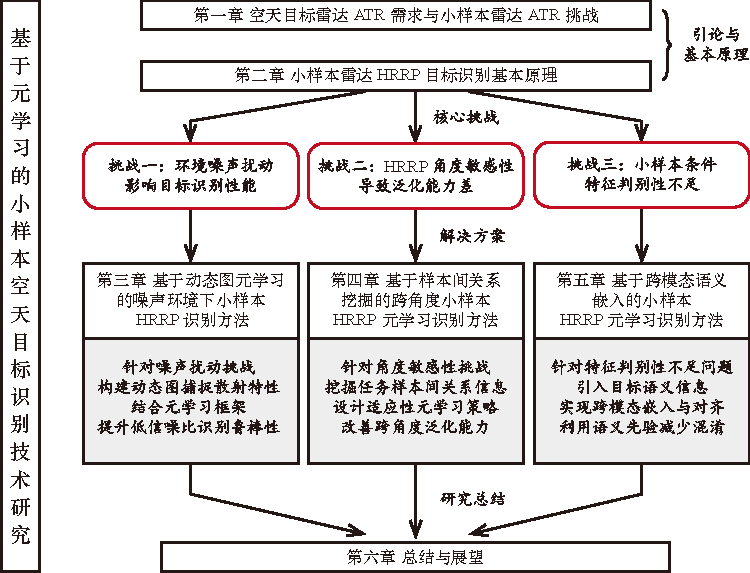
\includegraphics[width=0.95\linewidth]{figures/framework.pdf}
    \caption{本文组织架构和研究思路}
    \label{fig:framework}
\end{figure}

{第一章:绪论。} 作为开篇,本章首先阐明研究的宏观背景,即空天目标识别的重大国家战略需求;接着深入剖析RATR技术,包括其优势、固有局限以及当前发展趋势,并明确指出小样本问题是制约其发展的核心瓶颈;随后,对小样本RATR的研究现状、主要方法及面临的挑战进行综述,从而确立本论文的研究动机与定位;最后,概述本论文的主要研究工作和后续章节的内容安排。

{第二章:小样本雷达HRRP目标识别基本原理。} 本章为后续章节的研究提供必要的理论铺垫。内容包括:介绍宽带雷达成像与HRRP的基本原理、数学模型及其关键特性(如姿态敏感性);回顾基于深度学习的RATR框架;对小样本RATR问题进行形式化定义与分析,为后续提出基于元学习的解决方案奠定理论基础。

{第三章:基于动态图元学习的噪声环境下小样本HRRP识别方法。} 本章聚焦于第一个核心挑战:提升小样本HRRP识别的噪声鲁棒性。首先分析噪声对识别性能的影响机理。然后,详细阐述所提出的基于动态图元学习的识别方法,包括动态图构建策略、GNN表示学习模块、以及面向噪声鲁棒性的元学习框架设计与实现细节。最后,通过在含噪HRRP数据集上的仿真实验来验证方法的有效性,并与相关基线方法进行性能对比。

{第四章:基于样本间关系挖掘的跨角度小样本HRRP元学习识别方法。} 本章致力于解决第二个核心挑战:应对HRRP的角度敏感性。首先分析角度敏感性对小样本识别的制约。接着,详细介绍所提出的基于样本间关系挖掘的元学习方法,阐明如何利用图结构等机制建模样本间的角度关联,以及如何设计相应的元学习任务和优化策略来提升模型的角度泛化能力。最后,通过在具有角度变化的HRRP数据集上的实验,评估所提方法在跨角度小样本识别任务上的性能。

{第五章:基于跨模态语义嵌入的小样本HRRP元学习识别方法。} 本章旨在探索第三个核心方向:利用语义信息增强小样本HRRP识别。首先分析小样本下特征判别性不足的问题及引入语义的动机。然后,详细阐述融合跨模态语义嵌入的元学习方法,包括语义表示、HRRP特征提取(可能结合预训练模型)、跨模态融合机制、以及基于语义增强特征的元学习策略。最后,通过在含语义标签的HRRP数据集上的实验,验证该方法在提升小样本识别精度方面的效果。

{第六章:总结与展望。} 作为结尾,本章对全文的研究工作进行系统性总结,提炼主要的研究成果与创新点(即在利用元学习解决小样本HRRP识别的噪声鲁棒性、角度鲁棒性及语义融合问题上的贡献)。同时,客观地指出本研究存在的局限与待深入探讨的问题。最后,基于当前研究基础,对未来可能的研究方向进行展望。
